\documentclass[11pt, twoside]{report}
\usepackage[utf8]{inputenc}
\usepackage[T1]{fontenc}
\usepackage[spanish]{babel}


\usepackage[a4paper,width=150mm,top=25mm,bottom=25mm,bindingoffset=6mm]{geometry}
\usepackage{utopia}

\usepackage{glossaries}
\usepackage{hyperref}
\usepackage{booktabs}
\usepackage{cite}
\hypersetup{
    colorlinks=true,
    linkcolor=blue,
    filecolor=magenta,      
    urlcolor=cyan
}

\usepackage{graphicx}
\graphicspath{ {imagenes/} }


%%%%%%%%%%%%%%%%%%%%%%%%%%%%%%%%%%%%%%%
% Configuracion de formato de parrafos
\setlength{\parskip}{0.3em}
\renewcommand{\baselinestretch}{1.3}


%%%%%%%%%%
% Titulo %

%\title{Adopción de prácticas ágiles de desarrollo de software en los planes de estudio de universidades de Costa Rica\\
%	{\large Instituto Tecnológico de Costa Rica\\
%	Escuela de Ingeniería en Computación\\
%	Maestría en Computación\\
%	Ingeniería de Software
%	}
%}
%
%\author{Carlos Martín Flores González}
%
%\date{16 de Noviembre del 2017}


%%%%%%%%%%%%
% Glosario %


\makeglossaries


\newglossaryentry{unadeca}
{
    name=UNADECA,
    description={Universidad Adventista de Centro América}
}

\newglossaryentry{uam}
{
    name=UAM,
    description={Universidad Americana}
}

\newglossaryentry{ucem}
{
    name=UCEM,
    description={Universidad de Ciencias Empresariales}
}
 
\newglossaryentry{una}
{
    name=UNA,
    description={Universidad Nacional}
}

\newglossaryentry{ucr}
{
    name=UCR,
    description={Universidad de Costa Rica}
}

\newglossaryentry{uned}
{
    name=UNED,
    description={Universidad Estatal a Distancia}
}

\newglossaryentry{tec}
{
    name=TEC,
    description={Instituto Tecnológico de Costa Rica}
}

\newglossaryentry{ulacit}
{
    name=ULACIT,
    description={Universidad Latinoamerica de Ciencia y Tecnología}
}

\newglossaryentry{cenfotec}
{
    name=Cenfotec,
    description={Universidad Cenfotec}
}

\newglossaryentry{uaca}
{
    name=UACA,
    description={Universidad Autónoma de Centroamérica}
}

\newglossaryentry{invenio}
{
    name=Invenio,
    description={Universidad Invenio}
}

\newglossaryentry{uia}
{
    name=UIA,
    description={Universidad Internacional de las Américas}
}

\newglossaryentry{umca}
{
    name=UMCA,
    description={Universidad Metropolitana Castro Carazo}
}

\newglossaryentry{utn}
{
    name=UTN,
    description={Universidad Técnica Nacional}
}


\newglossaryentry{uisil}
{
    name=UISIL,
    description={Universidad Internacional San Isidro Labrados}
}


%%%%%%%%%%

\begin{document}



  
 
%\maketitle


\begin{titlepage}
    \begin{center}
        \vspace*{1cm}
        
        \Huge
        \textbf{Modelado y Simulación de Sistemas Distribuidos de Intercambio de Mensajes (\emph{Message Oriented Middleware})}
        
        \vspace{1.5cm}
        
        \textbf{Carlos Martín Flores González\\ \textnormal{\small{Carné: 2015183528}}}
        
        \vfill
        
        Profesor: César Garita
        
%        \vspace{0.5cm}
        
%        \includegraphics[width=0.4\textwidth]{university}
        
        \Large
        Instituto Tecnológico de Costa Rica\\
        Escuela de Ingeniería en Computación\\
        Maestría en Computación\\
        MC-7205 Tema Selecto de Investigación
        
        \vfill
        
        15 de Marzo del 2018
        
        
        
    \end{center}
\end{titlepage}




%%%%%%%%%%%
% Indices %

\pagenumbering{roman} 
\setcounter{page}{1}
\tableofcontents
\clearpage

%\listoffigures
%\cleardoublepage
%
\listoftables
\cleardoublepage

%%%%%%%%%%%%
% Prefacio %






%\addcontentsline{toc}{chapter}{Glosario}
%\printglossaries


\chapter*{Introducción}
\pagenumbering{arabic}
\addcontentsline{toc}{chapter}{Introducción}
Los métodos de predicción de rendimiento basados en modelos permiten a los arquitectos de software evaluar el rendimiento de los sistemas de software durante las primeras etapas de desarrollo. Estos modelos de predicción se centran en los aspectos relevantes de la arquitectura y de la lógica del negocio, dejando de lado detalles de la infraestructura subyacente. Sin embargo, estos detalles son esenciales para generar predicciones de rendimiento que sean precisas.

Para los ingenieros, es una práctica común simular el modelo de un artefacto antes de construirlo. Modelos de diseños de autos, circuitos electrónicos, puentes, entre otros, son simulados para entender el impacto de decisiones de diseño en varias atributos de calidad de interés como seguridad, consumo de energía o estabilidad. La habilidad de predecir las propiedades de un artefacto en base a su diseño sin necesidad de construirlo, es una de las características centrales de una disciplina de ingeniería. A partir de esta visión de lo que se considera una disciplina de ingeniería establecida se podría decir entonces que la ingeniería de software es apenas una disciplina de ingeniería. Esto porque frecuentemente los ingenieros de software carecen del entendimiento del impacto de decisiones de diseño en atributos de calidad como rendimiento o confiabilidad. Como resultado, se intenta probar la calidad del software mediante costosos ciclos de prueba y error.

El no entender el impacto en las decisiones de diseño puede ser costoso y riesgoso. Probar software significa que ya se ha hecho un esfuerzo en su implementación. Por ejemplo: si las pruebas revelan problemas de rendimiento, es muy probable que la arquitectura necesita ser modificada, lo que puede conllevar a costos adicionales. Estos costos surgen debido a que en sistemas de software empresarial un bajo rendimiento es principalmente el efecto de una arquitectura inadecuada que efecto de código.

%En los sistemas de software que utilizan comunicación basada en mensajes, el rendimiento depende en gran medida del \emph{middleware} orientado a intercambio de mensajes (\emph{Message Oriented Middleware} - MOM). Los arquitectos de software necesitan considerar su configuración y uso para obtener predicciones significativas. Sin embargo, la inclusión de un MOM en un modelo de arquitectura de software requiere un esfuerzo adicional así también como de conocimiento detallado de la infraestructura utilizada. Los arquitectos de software podrían llegar a omitir su influencia y esto tendría como consecuencia la generación predicciones erróneas.
%
%Las aplicaciones que utilizan protocolos de mensajería proporcionados por un MOM realizan comunicación asíncrona y basada en colas. Estas aplicaciones deben también hacer frente a consideraciones de arquitectura adicionales como la topología de las conexiones de los componentes, la persistencia de los mensajes y el flujo de control. Todos estos factores pueden llegar a influenciar en gran media el rendimiento de las aplicaciones. 



\textbf{Contribución - TBD}



\chapter{Definición del problema}
En los sistemas de software en los que se utiliza comunicación basada en mensajes, el rendimiento depende en gran medida del \emph{middleware} orientado a mensajes (\emph{Message Oriented Middleware} - MOM). Los arquitectos de software necesitan considerar su configuración y uso para obtener predicciones significativas sobre el comportamiento de la aplicación. Sin embargo, la inclusión de un MOM en un modelo de arquitectura de software requiere un esfuerzo adicional así también como de conocimiento detallado de la infraestructura utilizada. Los arquitectos podrían llegar a omitir la influencia del MOM y esto tendría como consecuencia la generación predicciones erróneas.

Las decisiones que han sido tomadas con poca información durante las etapas de diseño usualmente son muy difíciles de alterar y podrían hacer imposible el lograr los niveles requeridos de rendimiento de un sistema una vez que este haya sido puesto en producción. Es por esto que los arquitectos y diseñadores necesitan tener la habilidad de predecir el rendimiento del MOM utilizado, trabajando a partir de diseños abstractos sin tener acceso a la implemetación completa de la aplicación. Las aplicaciones que utilizan protocolos de mensajería proporcionados por un MOM realizan comunicación asíncrona y basada en colas. Estas aplicaciones deben también hacer frente a consideraciones de arquitectura adicionales como la persistencia de los mensajes y flujos de control. Todos estos factores pueden llegar a influenciar en gran media el rendimiento de las aplicaciones.

\chapter{Justificación}
El \emph{middleware} orientado a mensajes ha existido desde finales de los ochenta\cite{activemq-in-action}. No solo como un estilo de comunicación entre aplicaciones sino también como un estilo de integración. De esta forma, la mensajería cumple tanto necesidades para notificaciones así como de interoperabilidad entre aplicaciones. A través de los años, los sistemas han ido creciendo significativamente en complejidad y sofisticación. La necesidad de tener sistemas con mayor confiabilidad, escalabilidad y flexibilidad que en el pasado ha dado lugar a arquitecturas más complejas. En respuesta a esta creciente demanda por sistemas más rápidos, arquitectos, diseñadores y desarrolladores han hecho uso de los sistema de mensajería como una forma de resolver estos problemas complejos.

Actualmente, el uso de MOM  en arquitecturas de software modernas basadas microservicios, orientadas a eventos y de tipo \emph{Command-Query Responsability Segregation} (CQRS) es una solución popular que permite a las aplicaciones escalar con mayor facilidad y a la vez proporcionan integración en ambientes con tecnologías heterogeneas. Proveedores de servicios de computación en la nube como Amazon Web Services\footnote{Amazon Simple Queue Service(SQS) \url{https://aws.amazon.com/sqs/}}, Google Cloud Platform\footnote{Cloud Pub/Sub \url{https://cloud.google.com/pubsub/}} o Microsoft Azure\footnote{Queue Storage \url{https://azure.microsoft.com/en-us/services/storage/queues/}} disponen de soluciones de MOM.

Uno de los principales retos del MOM es el rendimiento\cite{alwakeel}. Muchas investigaciones se centran en el modelado de \emph{middleware} de comunicación y su rendimiento, pero diferentes aplicaciones tienen diferentes requerimientos y esto afecta el rendimiento. Los detalles del MOM subyacente son escenciales para un entendimiento y predicción de los sistemas de software que utilizan comunicación basada en mensajes. La configuración y el uso del MOM influye fuertemente en su rendimiento y en la utilización de recursos. En arquitecturas de software modernas como las mencionadas anteriormente, el MOM es una pieza muy importante. Su operación eficiente es crucial para las comunicaciones de misión crítica. Sin embargo el MOM puede degradarse o fallar debido a una variedad de razones, lo cual lo podría llegar a convertir en un cuello de botella dentro del sistema en donde se encuentre\cite{chew}.

El modelado de rendimiento es un enfoque útil para el análisis del rendimiento. Técnicas tradicionales de modelado de rendimiento pueden ser aplicadas a sistemas basadas en MOM\cite{liu-gordon}. Los modelos deben reflejar los efectos/comportamiento del MOM para permitir a los arquitectos de software evaluar la influencia en el rendimiento de la configuración de un MOM y de esta forma poder obtener predicciones sobre la influencia del MOM en el rendimiento del sistema.


A pesar de la importancia de contar con niveles satisfactorios de rendimiento, todavía hay una falta de enfoques de rendimiento que explícitamente tomen en cuenta las particularidades de una tecnología. Por ejemplo, en \cite{microservices-challenges} se menciona que aunque el rendimiento es una necesidad inherente para lograr escalabilidad y elasticidad, ingeniería de análisis de rendimiento para microservicios ha tenido muy poca atención. 

Con respecto a MOM, aunque se han publicado modelos de rendimiento sobre estos\cite{martince-et-al}, dichos modelos se han centrado más en el MOM como componente aislado y no como un componente más dentro de un sistema, es por esto que un estudio exploratorio para determinar la influencia del MOM en el rendimiento de un sistema podría arrojar nuevo conocimiento para dar a conocer factores que favorecen o desfavorecen el uso de estas tecnologías así como representar un nuevo cuerpo de conocimiento por medio del cual se pueda evaluar la adopción e impacto del MOM durante etapas de diseño. 


\chapter{Marco Teórico}

\section{\emph{Middleware} Orientado a Mensajes}

Junto con el crecimiento de Internet, los sistemas distribuidos han crecido a una escala masiva. Hoy en día, estos sistemas puede involucrar a miles de entidades distruidas globalmente. Esto ha motivado el estudio de modelos de comunicación y sistemas flexibles, que puedan reflejar la naturaleza dinámica y desacoplada de las aplicaciones.

La integración de tecnologías heterogéneas es una de las áreas principales en donde la comunicación basada en mensajes juega un papel clave. Más y más compañías se enfrentan al problema de integrar sistemas y aplicaciones heterogeneas dentro y fuera de la organización ya sea por fusiones, adquisiciones, requisitos comerciales o simplemente un cambio en la direción tecnológica. No es raro encontrar una gran cantidad de tecnologías y plataformas dentro de una solo compañía, desde productos de código libre y comerciales hasta sistemas y equipos heredados (\emph{legacy}).

La comunicación basada en mensajes también ofrece la habilidad de procesar solicitudes de manera asincrónica, proporcionando a los arquitectos y desarrolladores soluciones para reducir o eliminar cuellos de botella en un sistema e incrementar la productividad del usuario final y del sistema en general. Dado que la comunicación basada en mensajes provee un alto grado de desacoplamiento entre componentes, los sitemas que utilizan esta tecnología también logran contar con altos grados de agilidad y flexibilidad en su arquitectura.

A los sistemas de mensajería de aplicación-a-aplicación que se utilizan sistemas de negocios se les denomina genéricamente sistemas de mensajería empresarial o \emph{middleware} orientado a mensajes\cite{jms20}. MOM permite a dos o más aplicaciones intercambiar información en forma de mensajes. Un mensaje, en este caso, es un paquete autocontenido de datos de negocio y encabezados de enrutamiento de red. Los datos de negocio contenidos en un mensaje puede ser cualquier cosa, van a depender de cada negocio, y usualmente contiene información acerca de algún tipo de transacción. En sistemas de mensajería empresariales, los mensajes informan a una aplicación de la ocurrencia de algún evento en otro sistema. La tasa de mensajes depende de la capacidad de la implementación de MOM o \emph{broker}. El retraso depende de la latencia en el \emph{broker} y en los caminos de entrada y salida\cite{chew}.

Al usar MOM, los mensajes son trasmitidos desde una aplicación a otra a través de la red. Productos de \emph{middleware} empresarial aseguran que los mensajes se distribuyan correctamente entre las aplicaciones. Además estos productos usualmente proporcionan tolerancia a fallos, balanceo de carga, escalabilidad y soporte transaccional para sistemas que necesitan que necesitan intercambiar de manera confiable grandes cantidades de mensajes.

Los fabricantes de MOM usan diferentes formatos de mensajes y protocolos de red para intercambiar mensajes pero la semántica básica es la misma. Una interfaz de programación de aplicación (API, por sus siglas en inglés) se utiliza para crear un mensaje, cargar los datos, asignar información de enrutamiento y enviar el mensaje. La misma API se utiliza para recibir los mensajes producidos por otras aplicaciones.

En todos los sistemas modernos de mensajería empresarial, las aplicaiones intercambian mensajes a través de canales virtuales llamados destinos(\emph{destinations}). Cuando un mensaje se envía, se dirije a un destino (por ejemplo una cola o un tópico) no a una aplicación específica. Cualquier aplicación que subscriba o registre un interés en ese destino puede recibir el mensaje. De esta forma, las aplicaciones que reciben mensajes y aquellas que envían mensajes están desacopladas. Los emisores y receptores no están enlazados uno con otro de ninguna forma y pueden enviar y recibir mensajes como mejor les parezca.

Un concepto clave de MOM es que los mensajes son entregados de forma asincrónica desde un sistema a otros sobre la red. El entregar un mensaje de manera asicrónica significa que el emisor no requiere esperar a que el mensaje sea recibido o manejado por el receptor, él es libre de enviar el mensaje y continuar su procesamiento. Los mensajes asicrónicos son tratados como unidades autónomas: cada mensaje es autocontenido y lleva consigo todos los datos necesarios para ser procesado.

En comunicación de mensajes asincrónicos, las aplicaciones usan una API para contruir un mensaje, luego pasarlos al MOM para su entrega a uno o varios recipientes (Figura \ref{fig:mom}). Un mensaje es un paquete de datos que es enviado desde una aplicación a otra sobre la red. El mensaje debe de ser autodescriptivo en el sentido que debe de contener todo el contexto necesario para que permit a los recipientes llevar a cabo su trabajo de forma independiente. 


\begin{figure}[h]
  \centering
  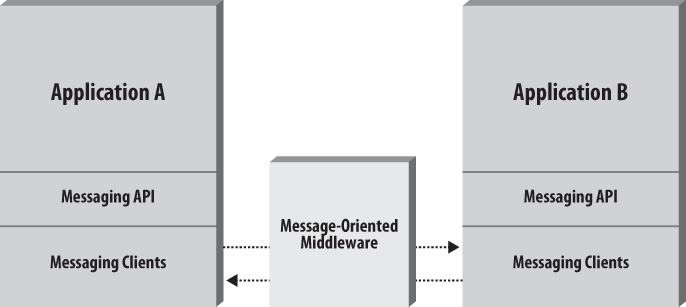
\includegraphics[width=10cm]{jms20-mom}
  \caption{\small{\emph{Middleware} Orientado a Mensajes. Tomado de \cite{jms20}}}
  \label{fig:mom}
\end{figure} 

La arquitecturas de MOM de hoy en día varían en su implementación. Van desde las arquitecturas centralizadas que dependen de un servidor de mensajes para realizar enrutamiento a arquitecturas descentralizadas que distribuyen el procesamiento del servidor hacia los clientes. Una variedad de protocolos como \texttt{TCP/IP, HTTP, SSL} y \texttt{IP} son empleados como capa de transporte de red.

Los sistemas de mensajería están compuestos por clientes de mensajería (\emph{messaging clients}) y algún tipo de servidos MOM. Los clientes envían mensajes el servidor de mensajería el cual distribuye estos mensajes a otros clientes. El cliente es una aplicación de negocio o componente que es usa una API de mensajería.

\subsection{Modelos de mensajería}

\subsubsection{Punto-a-Punto}
Este modelo de mensajería permite a los clientes enviar y recibir mensajes de forma sincrona como asíncrona a través de canales virtuales conocidos como colas. En este modelo a los productores de mensajes se les llama emisores (\emph{senders}) y a los consumidores se les conoce como receptores(\emph{receivers}). El modelo punto-a-punto ha sido tradicionalmente un modelo basado en \emph{polling}, en donde los mensajes son solicitados desde la cola en lugar de ser puestos en el cliente automáticamente. Los mensajes que se envían a una cola son recibidos por uno y solo un \emph{receiver}, aunque pueden haber otros \emph{receivers} escuchando en la cola por el mismo mensaje. Este es un modelo que promueve acoplamiento esto porque generalmente el \emph{sender} conocer cómo el mensaje va a ser utilizado y quién lo va a recibir. 

\subsubsection{\emph{Publish-and-Subscribe}}
En este modelo, los mesajes son publicados en un canal virtual llamado tópico. Los productores de mensajes son conocidos como \emph{publishers} y a los consumidores se les llama \emph{subscribers}. Los mensajes pueden ser recibidios por múltiples \emph{subscribers}, a diferencia del modelo punto-a-punto. Cada \emph{subscriber} recibe una copia de cada mensaje. Este es un modelo basado en \emph{push} en donde los mensajes son automáticamente transmitidos a los consumidores sin que estos tengan que solicitarlos o revisar la cola por nuevos mensajes. 

Este modelo tiende a ser menos acoplado que el modelo punto-a-punto debido a que el publicador del mensaje generalmente no está conciente de cuántos subscritores hay y lo que van a hacer estos con el mensaje.

\section{Ingeniería de rendimiento de software (\emph{Software Performance Engineering})}
La ingeniería de software tiene como objetivo tratar los retos de el proceso de desarrollo de software por mediante una disciplina de ingeniería. Una característica de esto es la disponibilidad de un catálogo de métodos y prácticas además de guías para la selección sistemática de estas prácticas. El objetivo ofrecer calidad, costo y plazos de entrega predecibles para el producto de ingeniería.

Un atributo no funcional que es usualmente es de alta importancia durante el desarrollo de software es el rendimiento del sistema en cuestión. Si los sistemas sufren de un rendimiento insuficiente, estos hace que usualmente no se utilicen como se esperaba o bien hacen que los proyectos fallen. Por lo tanto, la predicción del rendimiento de los sistemas de software está en el centro de agendas de investigación desde finales de los años noventa. El termino rendimiento a menudo  caracteriza el comportamiento en el tiempo y la eficiencia de los recursos de los sistema de hardware y de software. Las propiedades de rendimiento más importantes son tiempos de respuesta, \emph{throughput} y utilización de recursos.

La ingeniería de rendimiento de software (SPE, por sus siglas en inglés) se dedica a evaluar el rendimiento de sistemas de software al ofrecer diferentes métodos como modelado analítico, simulación y toma de mediciones. El objetivo de SPE es conducir evaluaciones del rendimiento de arquitecturas de software tan pronto como se pueda. 

En SPE, la creación y evaluación de modelos de rendimiento es un concepto centro para evaluar cuantitativamente el rendimiento del diseño de un sistema y predecir el rendimiento de otras alternativas de diseño. Un modelo de rendimiento captura el comportamiento relevante al rendimiento de un sistema para identificar el efecto de cambios en la configuración o en la carga de trabajo en el rendimiento. Permite predecir los efectos de tales cambios sin necesidad de implementarlo y ponerlo en producción, que podrían ser no solamente costoso sino también un desperdicio en el caso que un el hardware con el que se cuenta prueba ser insuficiente para soportar la intensidad de la carga de trabajo.

El punto de inicio de la mayoría de enfoques de SPE es la arquitectura del sistema de software. La arquitectura puede ser mejorada con anotaciones de rendimiento. Este modelo de software debe ser transformado en un modelo de rendimiento --como por ejemplo redes de colas, redes de Petri o cadenas de Markov -- para luego ser resuelto para las métricas de interés.

En el área de SPE, la idea de usar tecnologías orientadas a modelos ha ganado atención porque estas proporcionan transformación automática desde algún origen hacia un modelo de rendimiento. Sin embargo, los métodos de predicción de rendimiento basados en modelos requieren meta-modelos adecuados. Estos meta-modelos formalizan la sintáxis y semántica del modelo origen y destino. La transformación y procesamiento automático simplifica el enfoque de ingeniería de rendimiento de software y lo hace menos propenso a errores.

\subsection{Predicción de rendimiento dirigida por modelos}
La predicción del rendimiento dirigida por modelos permite a los arquitectos de software especificar modelos de rendimiento en un lenguaje especifico a su dominio. Esto puede a partir de modelos UML anotados con información relevante al rendimiento o por medio de lenguajes de descripción de arquitecturas especializados para la predicción de rendimiento como \emph{Palladio Component Model} (PCM). Para derivar métricas de rendimiento, el modelo de software se transforma en un modelo de rendimiento, como se muestra en la figura \ref{fig:model-driven-performance-prediction}. Las métricas de rendimiento derivadas del modelo de rendimiento deberían traducirse nuevamente al modelo de diseño, para permitir una interpretacio4n fácil para los arquitectos de software.

\begin{figure}[h]
  \centering
  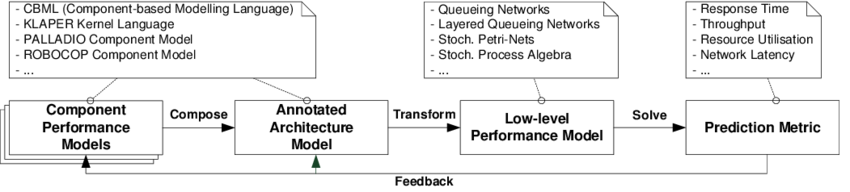
\includegraphics[width=15cm]{model-driven-performance-prediction}
  \caption{\small{Predicción de rendimiento dirigido por modelos.}}
  \label{fig:model-driven-performance-prediction}
\end{figure}

\section{Modelado de Arquitecturas de Software con el \emph{Palladio Component Model (PCM)}}
El \emph{Palladio Component Model} es un enfoque de modelaje para arquitecturas de software basados en componentes que permite predicción de rendimiento basada en modelos. PCM soporta el proceso de desarrollo de ingeniería basado en componentes y proporciona conceptos de modelaje para describir componentes de software, arquitectura de software, puesta en producción (\emph{deployment}) de componentes y perfiles de uso de sistemas de software basados en componentes en diferentes submodelos (Figura \ref{fig:pcm-instance}). 

\begin{figure}[h]
  \centering
  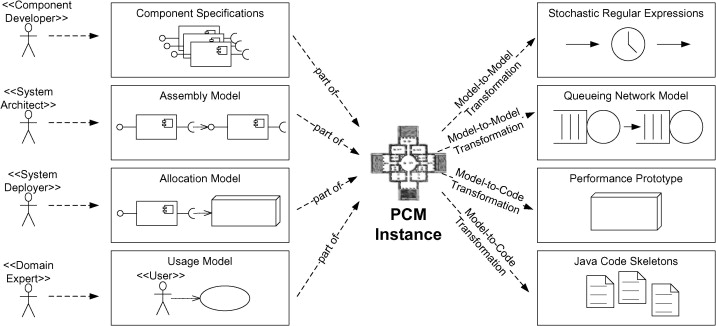
\includegraphics[width=15cm]{palladio-cbse-process}
  \caption{\small{Instancia de un modelo PCM}}
  \label{fig:pcm-instance}
\end{figure}

\begin{itemize}
    \item \textbf{Especificaciones de componentes} son descripciones abstractas y paramétricas de los componentes de software. En las especificaciones de software se proporciona una descripción del comportamiento interno del componente así como las demandas de sus recursos en RDSEFFs(\emph{Resource Demanding Service EFFect specifications}) utilizando una sintaxis similar a los diagramas de actividad de UML.
    \item \textbf{Un modelo de ensamblaje} (\emph{assembly model}) especifica qué tipo de componentes se utilizan en una instancia de aplicación modelada y si las instancias del component se replican. Además, define cómo las instancias del component se conectan representando la arquitectura de software.
    \item El entorno de ejecución y los recursos, así como el despliegue(\emph{deployment}) de instancias de componentes para dichos contenedores de recursos se definen en un \textbf{modelo de asignación}(\emph{allocation model}).
    \item El \textbf{modelo del uso} especifica la interacción de los usuarios con el sistema utilizando una sintaxis similar al diagrama de actividades de UML proporcionando una descripción abstracta de la secuencia y la frencuencia en que los usuarios activan las operaciones disponibles en un sistema.
\end{itemize}

Un modelo PCM abstrae un sistema de software a nivel de arquitectura y se anota con consumos de recursos que fueron medidos previamente u otros que son estimados. El modelo puede entonces ser usado en transformaciones de modelo-a-modelo o modelo-a-texto a un modelo de análisis en particular (redes de colas o simulación de código) que puede ser analiticamente resuelto o simulado para obtener resultados sobre el rendimiento y predicciones del sistema modelado. Los resultados del rendimiento y las predicciones pueden ser utilizadas como retroalimentación para evaluar y mejorar el diseño inicial, permitiendo así una evaluación de calidad de los sistemas de software en base a un modelo.

\chapter{Objetivos}

\section{Objetivo General}
Diseñar un modelo de sistemas distribuidos de intercambio mensajes (\emph{message-oriented middleware}) para evaluar la influencia que tienen en el rendimiento de un sistema de software por medio de modelado y simulación basado en componentes.

\section{Objetivos Específicos}
\begin{enumerate}
    \item \label{itm:obj1}Revisión del estado del arte de trabajos relacionados con enfoques de predicción y medición del rendimiento en sistemas de software basados en componentes y en \emph{middleware} orientado a mensajes
    \item \label{itm:obj2}Adaptar un sistema de software de referencia para el cual ya exista un modelo de rendimiento y simulaciones para que se integre y comunique con \emph{middleware} orientado a mensajes.
    \item \label{itm:obj3}Comparar la solución implementada bajo diferentes cargas de trabajo
    \item \label{itm:obj4}Crear un modelo del nuevo sistema y su rendimiento 
    \item \label{itm:obj5}Validar y analizar el modelo creado a través de experimentos
\end{enumerate}

\chapter{Entregables}

\section{Revisión de literatura}
\paragraph{Alineado con objetivo específico~\ref{itm:obj1}}

\paragraph{} Se pretende identificar los resultados de otros estudios relacionados como modelaje de rendimiento de software, así como retos y oportunidades de investigación que existan en esta área. Las preguntas de investigación que inicialmente propuestas para conducir esta revisión son las siguientes:
\begin{enumerate}
    \item[\textbf{PI1}] ¿Cuáles enfoques de predicción y medición del rendimiento en sistemas de software basados en componente se han propuesto?
    \item[\textbf{PI2}] ¿Cuáles enfoques de predicción y medición de rendimiento de software se han utilizado para \emph{middleware} orientado a mensajes?    
    \item[\textbf{PI3}] ¿Qué retos y oportunidades existen con estos enfoques en la actualidad?
    \item[\textbf{PI4}] ¿Qué herramientas hay disponibles para modelodo, rendimiento...
\end{enumerate}


\section{Aplicación adaptada para que soporte comunicación basada en mensajes}
\paragraph{Alineado con objetivos específicos~\ref{itm:obj2} y \ref{itm:obj3}}  

\paragraph{}Una vez que se haya identificado un sistema de software del cual ya exista un modelo de rendimiento y simulaciones, este se tomará como base para adaptarlo de tal forma que utilice \emph{middleware} orientado a mensajes en algún punto de su ejecución.

A la aplicación adaptada se le realizarán mediciones de su rendimiento con el fin de tener estos como entrada para las subsecuentes tareas de modelado propuestas. Serán estas mediciones las que ayudan a refinar y calibrar el modelo.

\section{Modelo de rendimiento del nuevo sistema}
\paragraph{Alineado con objetivos específicos~\ref{itm:obj4} y \ref{itm:obj5}}

\paragraph{}A partir del sistema adaptado y sus mediciones, se modificará el modelo de rendimiento original del sistema de referencia para reflejar los cambios introducidos por el \emph{middleware} orientado a mensajes.

Este nuevo modelo se ejercitará con los perfiles de uso de la aplicación de referencia, con el fin de validar si este puede aproximar el comportamiento del sistema ahora que se le han introducido cambios. 

\chapter{Cronograma}

\bibliographystyle{ACM-Reference-Format}
\begin{thebibliography}{9}

\bibitem{performance-model-survey} Heiko Koziolek. 2010. \emph{Performance evaluation of component-based software systems: A survey. Perform}. Eval. 67, 8 (August 2010), 634-658. DOI: \url{http://ezproxy.itcr.ac.cr:2075/10.1016/j.peva.2009.07.007} 

\bibitem{palladio-seminal} Stephen Becker, Heiko Koziolek and Ralf Reussner. \emph{The Palladio component model for model-driven prediction}. Journal of Systems and Software 82:3-22. Elsevier Science Inc. 2009. DOI: \url{http://dx.doi.org/10.1016/j.jss.2008.03.066}

\bibitem{performance-devops} Andreas Brunnert, André van Hoorn, Felix Willnecker, Alexandru Danciu, Wilhelm Hasselbring, Christoph Heger, Nikolas Roman Herbst, Pooyan Jamshidi, Reiner Jung, Jóakim von Kistowski, Anne Koziolek, Johannes Kroß, Simon Spinner, Christian Vögele, Jürgen Walter, and Alexander Wert. \emph{Performance-oriented devops: A research agenda}. Technical Report SPEC-RG-2015-01, SPEC Research Group - DevOps Performance Working Group, Standard Performance Evaluation Corporation (SPEC), 2015. \url{http://arxiv.org/abs/1508.04752}

\bibitem{microservices-challenges} Robert Heinrich, André van Hoorn, Holger Knoche, Fei Li, Lucy Ellen Lwakatare, Claus Pahl, Stefan Schulte, and Johannes Wettinger. \emph{Performance engineering for microservices: Research challenges and directions}. In Companion Proceedings of the 8th ACM/SPEC on International Conference on Performance Engineering, 2017, pages 223-226. DOI: \url{https://doi.org/10.1145/3053600.3053653}

\bibitem{case-study-1} Thijmen de Gooijer, Anton Jansen, Heiko Koziolek, and Anne Koziolek. 2012. \emph{An industrial case study of performance and cost design space exploration}. In Proceedings of the 3rd ACM/SPEC International Conference on Performance Engineering (ICPE '12). ACM, New York, NY, USA, 205-216. DOI: \url{https://ezproxy.itcr.ac.cr:2878/10.1145/2188286.2188319}

\bibitem{huber-et-al} Nikolaus Huber, Steffen Becker, Christoph Rathfelder, Jochen Schweflinghaus, and Ralf H. Reussner. 2010. \emph{Performance modeling in industry: a case study on storage virtualization}. In Proceedings of the 32nd ACM/IEEE International Conference on Software Engineering - Volume 2 (ICSE '10), Vol. 2. ACM, New York, NY, USA, 1-10. DOI: \url{http://ezproxy.itcr.ac.cr:2075/10.1145/1810295.1810297} 

\bibitem{rathfelder-et-al} Christoph Rathfelder, Steffen Becker, Klaus Krogmann and Ralf Reussner. \emph{Workload-aware System Monitoring Using Performance Predictions Applied to a Large-scale E-Mail System}. 2012 Joint Working IEEE/IFIP Conference on Software Architecture and European Conference on Software Architecture, Helsinki, 2012, pp. 31-40.
DOI: \href{https://ezproxy.itcr.ac.cr:2878/10.1109/WICSA-ECSA.212.11}{10.1109/WICSA-ECSA.212.11}. 

\bibitem{media-store} Misha Strittmatter and Amine Kechaou. \emph{The media store 3 case study system}. Technical Report 2016,1, Faculty of Informatics, Karlsruhe Institute of Technology, 2016. URL: \url{http://digbib.ubka.uni-karlsruhe.de/volltexte/documents/3792054}

\bibitem{activemq-in-action} Bruce Snyder, Dejan Bosnanac, Rob Davies. \emph{ActiveMQ in Action}. Manning, 2011. 

\bibitem{alwakeel} S.S. Alwakeel and H.M. Almansour. \emph{Modeling and Performance Evaluation of Message-oriented Middleware with Priority Queuing}. Information Technology Journal, 10: 61-70. 2011. DOI \url{http://dx.doi.org/10.3923/itj.2011.61.70}

\bibitem{chew} Chew, Zen Bob. \emph{Modelling Message-oriented-middleware Brokers Using Autoregressive Models for Bottleneck Prediction}. PhD Thesis. Queen Mary, University of London. 2013. \url{https://qmro.qmul.ac.uk/jspui/handle/123456789/8832} 

\bibitem{liu-gordon} Yan Liu and Ian Gorton. \emph{Performance prediction of J2EE applications using messaging protocols}. In Proceedings of the 8th international conference on Component-Based Software Engineering (CBSE'05), George T. Heineman, Ivica Crnkovic, Heinz W. Schmidt, Judith A. Stafford, and Clemens Szyperski (Eds.). Springer-Verlag, Berlin, Heidelberg, 1-16. 2005. DOI \url{http://ezproxy.itcr.ac.cr:2075/10.1007/11424529_1}

\bibitem{jms20} Mark Richards, Richard Monson-Haefel, David Chappell. \emph{Java Message Service}. O'Reilly Media. Segunda Edición. 2009.

\bibitem{martince-et-al} Tomáş Martinec, Lukáş Marek, Antonín Steinhauser, Petr Tůma, Qais Noorshams, Andreas Rentschler, and Ralf Reussner. \emph{Constructing performance model of JMS middleware platform}. In Proceedings of the 5th ACM/SPEC international conference on Performance engineering (ICPE '14). ACM, New York, NY, USA, 123-134. 2014. DOI: \url{https://ezproxy.itcr.ac.cr:2878/10.1145/2568088.2568096}

\end{thebibliography}







%\addcontentsline{toc}{chapter}{Resumen}
%\chapter*{Resumen}
%A pesar de la popularidad de las metodologías ágiles de desarrollo de software en la industria, expresada en varias encuestas y estudios recientes, muchas organizaciones siguen reportando en estas mismas encuestas que se cuenta con poco personal capacitado con las habilidades necesarias y que los planes de estudio de carreras de tecnología de información muestran rezagos en estos temas. Con el fin de brindar una formación que no solamente incluya la enseñanza de prácticas ágiles sino también el desarrollo de otras actitudes como el trabajo en equipo y el empredurismo, las universidades han venido introduciendo paulativamente estas prácticas a sus planes de estudio principalmente por medio de enfoques de \emph{aprender-haciendo}. Universidades en Costa Rica también han reportado la inclusión de estos temas en sus planes de estudio como respuesta a las tendencias mundiales y para apoyar la creciente industria de desarrollo de software del país.
%
%
%\addcontentsline{toc}{section}{\emph{Abstract}}
%\section*{\emph{Abstract}}
%Despite the popularity of the agile engineering practices in the software industry reported in recent surveys and studies, many organizations keep reporting in those same surveys which they have no enough personal with the desired skill set, and also that they think that IT curricula is behind in these new software development trends. In order to provide an education which involves agile engineering practices but also other skills such as teamwork and entrepreneurship, universities have been introducing these practices in their curricula, mainly by the use of \emph{learning-by-doing} approaches. Universities in Costa Rica have reported the introduction of these topics in their curricula as a response to their increasing popularity and to support the growing software industry in the country.  
%
%\addcontentsline{toc}{section}{\emph{Palabras Clave / Keywords}}
%\subsection*{Palabras Clave / Keywords}
%agile software development, agile teaching, agile engieering practices, software engineering education, costa rica software education


%%%%%%%%%%%%%
% Capitulos %

%\chapter*{Introducción}
%\pagenumbering{arabic}
%\addcontentsline{toc}{chapter}{Introducción}
%\input{capitulos/introduccion}
%
%\chapter{Generalidades de la Investigación}
%\input{capitulos/ch1}
%
%\chapter{Marco Teórico} \label{ch2:marco-teorico}
%\input{capitulos/ch2}
%
%\chapter{Marco Metodológico}
%\input{capitulos/ch3}
%
%
%\chapter{Resultados Esperados}
%\input{capitulos/ch4}
%
%\chapter{Plan de Trabajo}
%\input{capitulos/ch5}
%
%% Bibliografia
%\addcontentsline{toc}{chapter}{Bibliografía}
%\input{capitulos/bibliografia}
%
%\addcontentsline{toc}{chapter}{Apéndice}
%\chapter*{Apéndice}
%\input{capitulos/apendice}

%Portada
% 
% 
%\frontmatter
% 
%\addcontentsline{toc}{chapter}{Forewordq}
%hola
% 
%\addcontentsline{toc}{chapter}{Dummy entry}
%Some text...
% 
%\tableofcontents
% 
%\mainmatter
% 
%\chapter{First Chapter}
% 
%This will be an empty chapter...
 
\end{document}

